\label{sec:Lp}

\subsection{$l_{p}$ norm} Now we have overviewed the works based on $l_0$ and $l_1$ norm, how about the other values of $p$?

In fact, \cite{elad2010sparse} has given a brief discussion about it when $0<p<1$ and illustrate the tendency of $l_{p}$($0<p<1$) norm to drive results to become sparse. Then base on recent advances in sparsity-inducing penalties\cite{bach2012optimization,marjanovic2012optimization} that have been successfully applied in compressive sensing\cite{candes2008introduction}, \cite{bouaziz2013sparse} expresses the ICP registration problem as a sparse $l_{p}$ optmization$0\leq p\leq1$, obtain an heuristic-free, robust rigid registration algorithm. And \cite{chartrand2007exact} showing that $l_{p}$ norms with $p<1$ outperform the $l_1$ norm in inducing sparsity makes the optimization more resilient to a large number of outliers. Figure...is the registration results of sparse ICP under different values of $p$ among which it can be found that $0<p<1$ gives the best result, but how to automatically decide $p$ is not discussed.

\begin{figure}[ht]
  \centering
  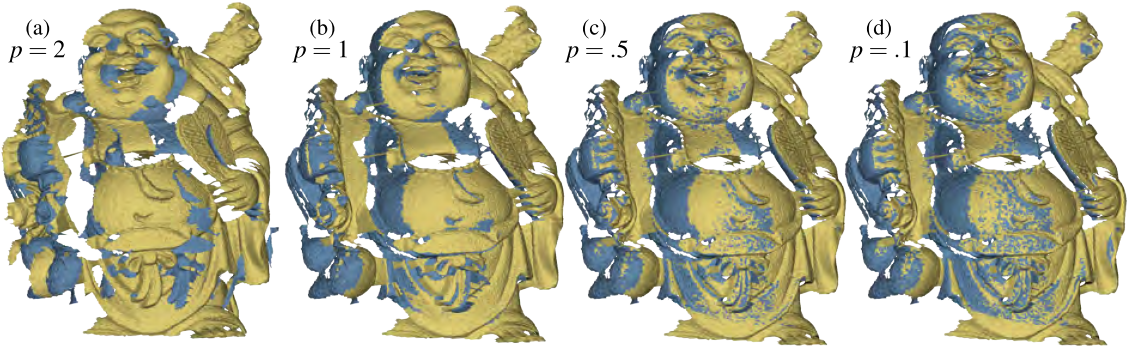
\includegraphics[width=3in]{images/sparseICP}
  \caption{$l_{p}$ optimization: registration using sparse ICP\cite{chartrand2007exact}.}
\end{figure}

In addition, there is still another kind of promotion for sparse representation. Sparse Subspace Clustering(SSC) \cite{elhamifar2009sparse} introduces compressed sensing techniques to subspace segmentation. SSC uses the sparsest representation produced by $l_1$ optimization to define the affinity matrix of an undirected graph. It is based on the observation that each point in a union of linear subspaces can always be represented as a linear combination of the points belonging to the same linear subspace. Inspired by SSC and \cite{cheng2011multi}, \cite{hu2012co} proposes a subspace clustering formulation of optimization with a consistent multi-feature penalty achieved with both $l_{2,1}$ norm and $l_{1,1}$ norm to guarantee the consistency of co-segmentation results according to various features. Briefly, after over-segmenting the input models into primitive patches(left in Figure...), they group the similar patches via a subspace clustering scheme. Figure...(right) is the co-segmentation result.

\begin{figure}[ht]
  \centering
  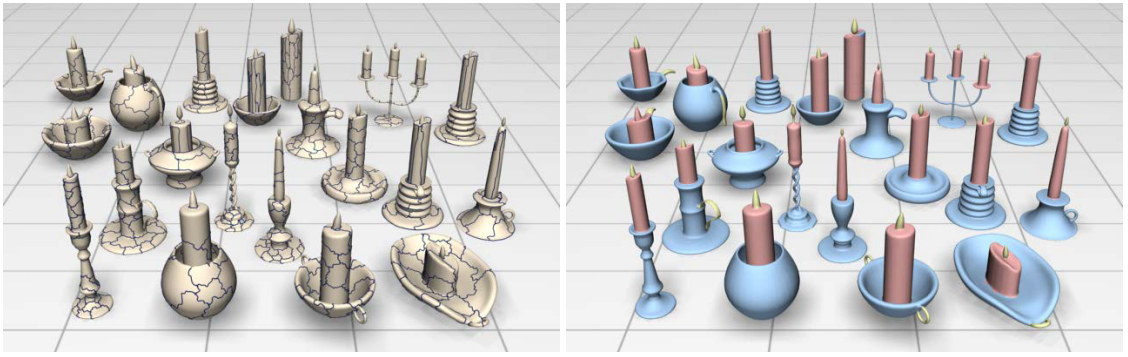
\includegraphics[width=3in]{images/co-segmentation}
  \caption{$l_{p}$ optimization: co-segmentation\cite{hu2012co}. Left: over segmented patches. Right: co-segmented result.}
\end{figure} 